\section{Case Studies}
\label{sec:casestudies}

Four production-ready NormCode plans are mentioned in the paper, each encoding a distinct
orchestration class as a Level~2 case: \textbf{PPT Generation} (${\sim}30$ inferences;
nested loop, 6 layouts, 14 component types), \textbf{Code Assistant} (${\sim}40$;
ReAct outer loop with parallel Explore), \textbf{NC~Compilations} (${\sim}25$;
self-hosting Level~2 validation --- the compiler is itself a NormCode plan), and
\textbf{Canvas Assistant} (${\sim}20$; built-in chat controller with natural-language
command dispatch). Syntactic nodes constitute 60--70\% of total inferences across all
plans. NC~Compilations has been successfully executed end-to-end with
qwen-plus, producing correct repositories for plans such as report writing and contract reviewing.
The other two of the four plans are traced in detail below.

\begin{figure}[!htbp]
  \centering
  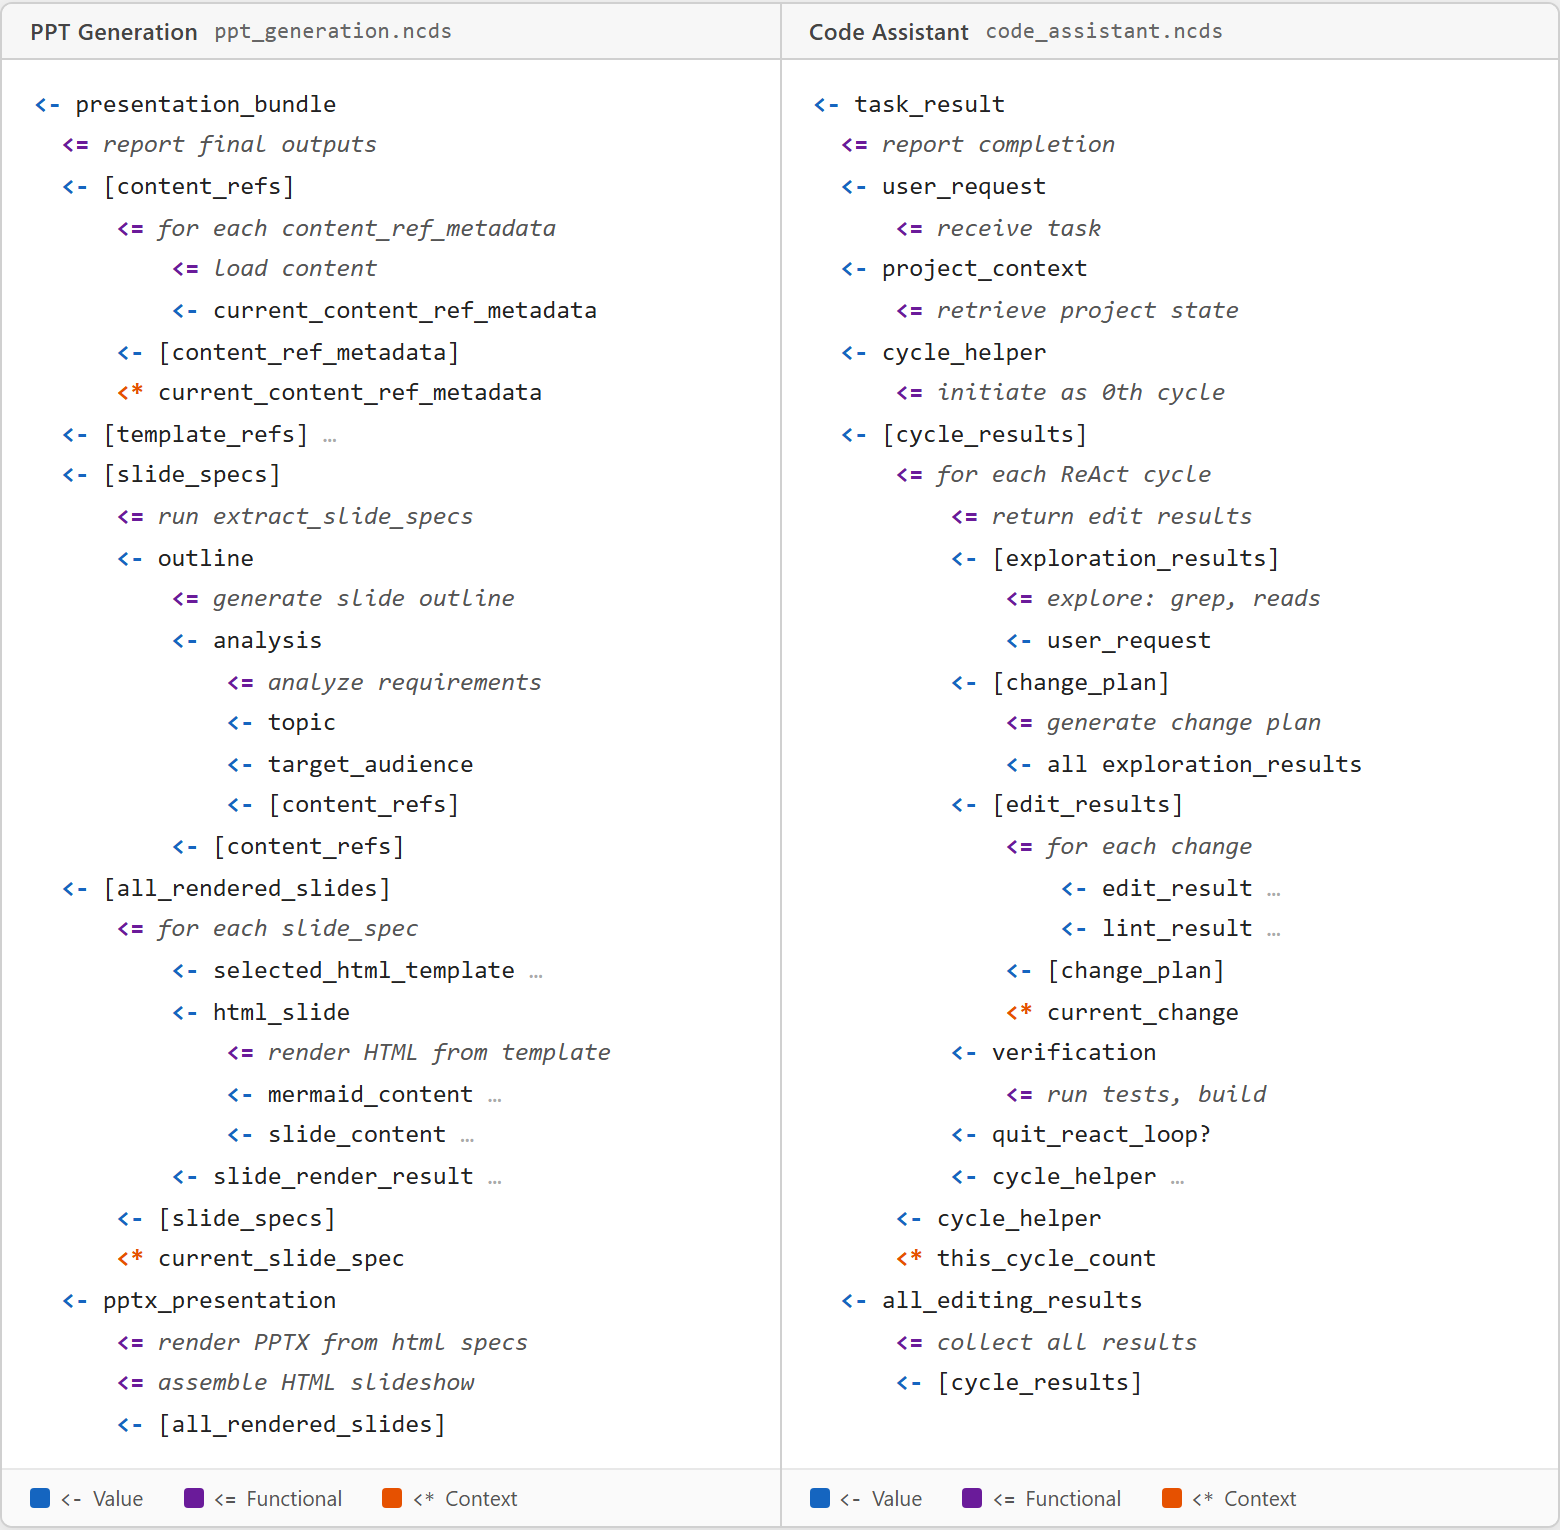
\includegraphics[width=\textwidth]{figures/ppt_and_code_ncs.png}
  \caption{PPT Generation (left) and Code Assistant (right) as Level~2 cases
    (\texttt{.ncds}, abbreviated).
    Left: nested dual-output loop (HTML + PPTX per slide).
    Right: ReAct outer loop \cite{yao2023} with inner explore, plan, edit, and verify stages.
    \textcolor{blue}{\texttt{<-}} Value; \textcolor{violet}{\texttt{<=}} Functional;
    \textcolor{orange}{\texttt{<*}} Context.}
  \label{fig:plans}
\end{figure}

\subsection{Case Study 1: PPT Agent --- Level 2 Reuse and Level 1 Accumulation}

\texttt{ppt\_generation.ncds} (Fig.~\ref{fig:plans}, left) is a Level~2 case encoding
a parallel dual-output pipeline: HTML and PPTX slides are generated from the same
componentized content JSON per slide. The most expensive semantic nodes are
\texttt{generate componentized content} and \texttt{generate diagram code};
the remainder run with negligible cost and a total latency around 5 minutes with
visible intermediate steps. The production plan uses Chinese concept names throughout
(Fig.~\ref{fig:ppt}); the compiler and orchestrator are agnostic to natural language.
Reusing a checkpoint requires the referenced files or APIs to remain accessible ---
the case encodes \textit{what} was used, not its content.

\begin{figure}[!htbp]
  \centering
  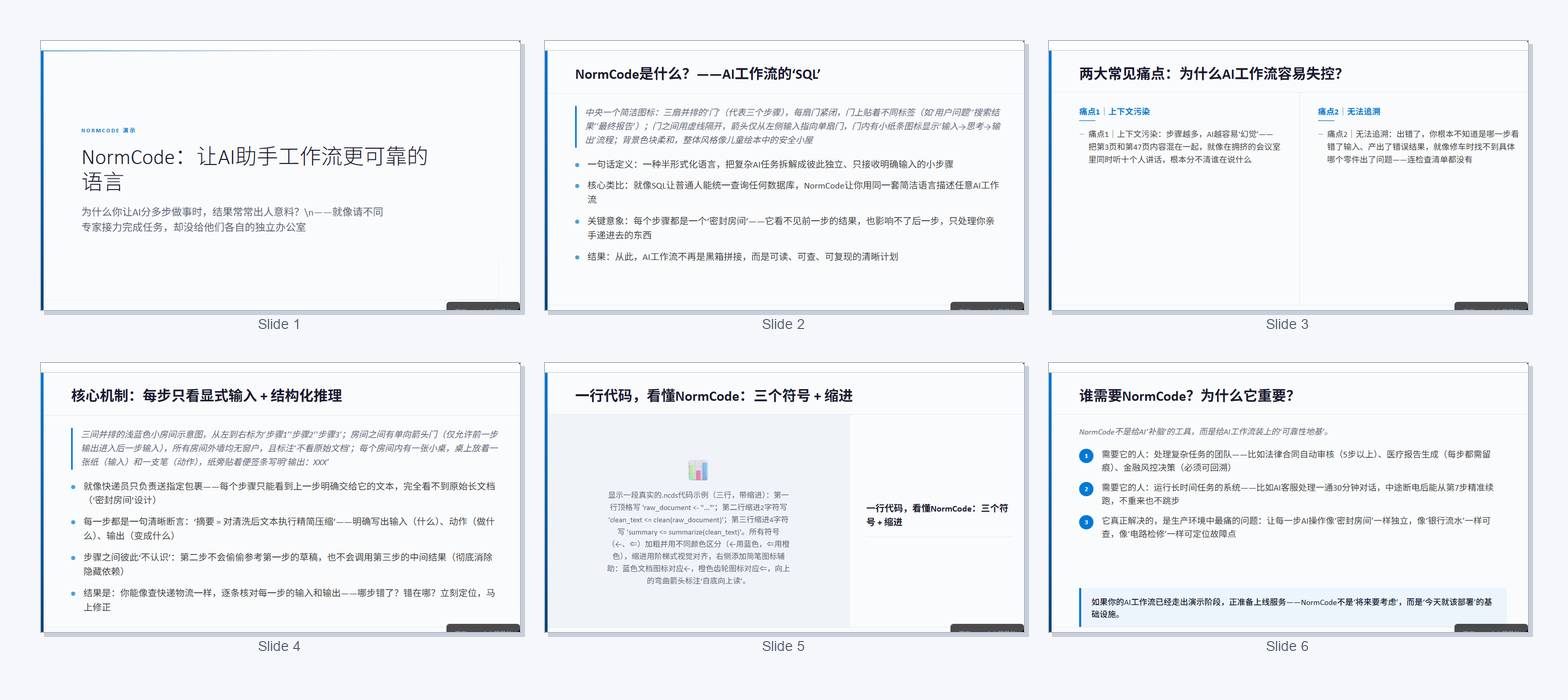
\includegraphics[width=\textwidth]{figures/fig4.png}
  \caption{Six slides produced by the PPT Generation plan (Chinese-language run).
    Each slide is a Level~1 checkpoint accumulated during execution.}
  \label{fig:ppt}
\end{figure}

\subsection{Case Study 2: Code Assistant --- A ReAct Plan as a Level~2 Case}

\texttt{code\_assistant.ncds} (Fig.~\ref{fig:plans}, right) is a Level~2 case encoding
a ReAct-loop software engineering workflow \cite{yao2023}. Each cycle, Explore
\textit{observes} (parallel file reads, zero LLM cost), Plan \textit{reasons} (one LLM
call over scoped exploration results), Implement \textit{acts} (surgical edits with an
inner lint-fix loop), and Verify checks results. Implement receives the change plan,
not the raw file contents from Explore --- scope isolation in action. Every run
generates a Level~1 case base: every stage is a checkpoint, and the Canvas App
makes each one inspectable and revisable (Sect.~\ref{sec:canvas}).

